%%%%%%%%%%%%%%%%%%%%%%%%%%%%%%%%%%%%%%%%%
% Plasmati Graduate CV
% LaTeX Template
% Version 1.0 (24/3/13)
%
% This template has been downloaded from:
% http://www.LaTeXTemplates.com
%
% Original author:
% Alessandro Plasmati (alessandro.plasmati@gmail.com)
%
% License:
% CC BY-NC-SA 3.0 (http://creativecommons.org/licenses/by-nc-sa/3.0/)
%
% Important note:
% This template needs to be compiled with XeLaTeX.
% The main document font is called Fontin and can be downloaded for free
% from here: http://www.exljbris.com/fontin.html
%
%%%%%%%%%%%%%%%%%%%%%%%%%%%%%%%%%%%%%%%%%

%----------------------------------------------------------------------------------------
%	PACKAGES AND OTHER DOCUMENT CONFIGURATIONS
%----------------------------------------------------------------------------------------

\documentclass[10pt]{report} % Default font size and paper size
\usepackage[top=1cm,bottom=1cm,margin=2cm]{geometry}
%\geometry{top=1cm,bottom=1cm,margin=1cm}
\usepackage[breaklinks=true]{hyperref}

%\usepackage{fontspec} % For loading fonts
%\defaultfontfeatures{Mapping=tex-text}
%\setmainfont[SmallCapsFont = Fontin SmallCaps]{Fontin} % Main document font


%\usepackage{xunicode,xltxtra,url,parskip} % Formatting packages
\usepackage{url,parskip}

\usepackage[usenames,dvipsnames]{xcolor} % Required for specifying custom colors

%\usepackage{fullpage}
%\usepackage[big]{layaureo} % Margin formatting of the A4 page, an alternative to layaureo can be 
%\usepackage{fullpage}
% To reduce the height of the top margin uncomment: \addtolength{\voffset}{-1.3cm}
%\addtolength{\voffset}{-0.8cm}

\usepackage{hyperref} % Required for adding links	and customizing them
\definecolor{linkcolour}{rgb}{0,0.2,0.6} % Link color
\hypersetup{colorlinks,breaklinks,urlcolor=linkcolour,linkcolor=linkcolour} % Set link colors throughout the document

\usepackage{titlesec} % Used to customize the \section command
\titleformat{\section}{\Large\scshape\raggedright}{}{0em}{}[\titlerule] % Text formatting of sections
\titlespacing{\section}{0pt}{3pt}{3pt} % Spacing around sections

\usepackage{titlesec}
\titleformat{\chapter}[display]
{\normalfont\bfseries}{}{0pt}{\huge}


\makeatletter
\renewcommand{\@makechapterhead}[1]{%
	{\noindent\raggedright\normalfont% Alignment and font reset
		\huge\bfseries \thechapter~~#1\par\nobreak}% Formatting
	\vspace{\baselineskip}% ...just a little space
}
\makeatother



%
%\makeatletter
%\newcommandtwoopt{\citeads}[3][][]{\href{http://adsabs.harvard.edu/abs/#3}%
%	{\def\hyper@linkstart##1##2{}%
%		\let\hyper@linkend\@empty\citealp[#1][#2]{#3}}}
%\newcommandtwoopt{\citepads}[3][][]{\href{http://adsabs.harvard.edu/abs/#3}%
%	{\def\hyper@linkstart##1##2{}%
%		\let\hyper@linkend\@empty\citep[#1][#2]{#3}}}
%\newcommandtwoopt{\citetads}[3][][]{\href{http://adsabs.harvard.edu/abs/#3}%
%	{\def\hyper@linkstart##1##2{}%
%		\let\hyper@linkend\@empty\citet[#1][#2]{#3}}}
%\newcommandtwoopt{\citeyearads}[3][][]%
%{\href{http://adsabs.harvard.edu/abs/#3}
%	{\def\hyper@linkstart##1##2{}%
%		\let\hyper@linkend\@empty\citeyear[#1][#2]{#3}}}
%\makeatother

\renewcommand{\contentsname}{Table des mati\`eres}


\begin{document}

\tableofcontents

\newpage

%\font\fb=''[cmr10]'' % Change the font of the \LaTeX command under the skills section

%----------------------------------------------------------------------------------------
%	NAME AND CONTACT INFORMATION
%----------------------------------------------------------------------------------------

\vspace{-4cm}

\chapter{Curriculum Vitae} \label{CV} 

%\par{\centering{\Huge Curriculum Vitae - Etienne \textsc{Bonnassieux}\label{CV}}\bigskip\par} % Your name
\vspace{-0.2cm}
%%\section{Personal Information}
%\hspace{-0.5cm}
%\begin{tabular}{rl}
%\textsc{Born:} & Noisy-le-Sec  | 19/10/1991 \\
%\textsc{Address:} & 15 Rue Lakanal, 75015 Paris \\
%\end{tabular}
%\hspace{2cm}
\begin{center}
\begin{tabular}{rl|rl}
\textsc{Date de naissance:} & 19/10/1991 &
\textsc{email:} & \href{mailto:etienne.bonnassieux@obspm.fr}{etienne.bonnassieux@uni-wuerzburg.de}\\
\textsc{Lieu de naissance:} &Noisy-le-Sec &
\textsc{Phone:} & +33 6 95 98 33 20
\end{tabular}
\end{center}

\vspace{0.3cm}

%----------------------------------------------------------------------------------------
%	COLLABS
%----------------------------------------------------------------------------------------

Mes thématiques de recherche concernent l’étude \`a basses radiofréquences ($\sim30-144$\,MHz) et haute résolution angulaire (sub-arcsec), de la formation et l’évolution des galaxies, de leurs noyaux actifs, et de grandes structures comme les amas de galaxies et les filaments cosmiques avec  l'instrument LOFAR (\textit{LOw Frequency ARray}), et son extension française \textit{NenuFAR} et plus tard \textit{SKA}. J’ai développé une compétence technique et observationnelle en VLBI (\textit{Very Long Baseline Interferometry}) et en radiointerférométrie avancée, adaptée à l’ère \textit{SKA}, permettant la mise en {\oe}uvre de nouvelles techniques et modes d’utilisation de réseaux interféromètriques.




\section{Positions de recherche}

\begin{tabular}{r|p{15.5cm}}
	\textsc{F\'ev 2022} & Poste post-doctoral, portant sur l'\'etude des jets relativistes de blazars avec LOFAR, \`a la \textit{Julius-}\\
	\textsc{Pr\'esent}&\textit{ Maximilians-Universit{\"a}t} de W{\"u}rzburg, Allemagne, sous la supervision de Matthias Kadler dans le cadre du financement \hyperlink{https://www.for5195.uni-wuerzburg.de/}{DFG-FOR5195} en cotutelle avec l'Universit\'e de Hambourg.\\
	\multicolumn{2}{c}{} \\
	\textsc{Oct 2018} & Poste post-doctoral \`a l'Universit\'e de Bologne portant sur l'\'etude des amas de galaxies \`a basses \\
	\textsc{F\'ev 2022}& fr\'equences avec LOFAR, sous la direction d'Annalisa Bonafede dans le cadre de \hyperlink{https://cordis.europa.eu/project/id/714245}{l'ERC DRANOEL}.\\
	\multicolumn{2}{c}{} \\
\end{tabular}


\section{Collaborations internationales pr\'esentes}

\begin{tabular}{r|p{15.5cm}}
	
	\textsc{F\'ev 2022} & \textbf{Unit\'e de recherche DFG: ``Jets Relativistes dans les Galaxies Actives" (Allemagne)}\\
	\textsc{Pr\'esent}  & Employeur actuel. Je travaille sp\'ecifiquement sur l'\'etude de jets blazars \`a larges \'echelles, et ce que nous r\'ev\`elent les observations radios \`a basses fr\'equences sur leur \'emission hautes-\'energies.\\
	\multicolumn{2}{c}{} \\

	
\textsc{Oct 2015} & \textbf{Key Science Projects (KSPs) de LOFAR: Relev\'es et Magn\'etisme (International)}\\
\textsc{Pr\'esent}  &  Groupes de travail : \textbf{Relev\'es}: cartographie le ciel radio Nord \`a 144\,MHz et 60\,MHz. \textbf{Magn\'etisme}: \'etude de la distribution du champ magn\'etique mesur\'e par LOFAR.\\
\multicolumn{2}{c}{} \\

	\textsc{Oct 2017} & \textbf{NenuFAR (France)}\\
	\textsc{Pr\'esent}  & Extension basse-$\nu$ Fran\c{c}aise de LOFAR; je suis le PI du programme long-terme LT09 "Filaments d'amas \& Magn\'etisme Cosmique".\\
	\multicolumn{2}{c}{} \\
	
	\textsc{Oct 2017} & \textbf{Groupe de travail LOFAR-VLBI (International)}\\
	\textsc{Pr\'esent}  &  But: rendre possible, puis faciliter l'utilisation de l'International LOFAR Telescope (r\'esolution sub-arcseconde \`a 144\,MHz).\\
	\multicolumn{2}{c}{} \\
	
	\textsc{Jan 2024} & \textbf{Groupe de trravail SKA-VLBI (International)}\\
	\textsc{Pr\'esent}  &  But: d\'evelopper de futures capacit\'es VLBI pour le SKA.\\
	\multicolumn{2}{c}{} \\
	

	
	%------------------------------------------------
\end{tabular}

%----------------------------------------------------------------------------------------
%	EDUCATION
%----------------------------------------------------------------------------------------

\section{\'Education \& Qualifications}

\begin{tabular}{r|p{15.5cm}}
	\textsc{Jan 2020} & \textbf{Qualification CNU}\\
	& Section 34.\\
	\multicolumn{2}{c}{} \\

\textsc{2015-2018} & \textbf{Doctorat en Astrophysique} - \textit{Observatoire de Paris $\&$ Rhodes University, Afrique du Sud}\\
& Supervisors: Philippe Zarka, Oleg Smirnov, Cyril Tasse. \textbf{Obtenue en Septembre 2018.}\\
& ``Analyse statistique de l’\'Equation de la Mesure Radio-Interférométrique, un schéma de pondération en découlant, et des applications à une observation LOFAR-VLBI de l’\textit{Extended Groth Strip}"\\
& Co-tutelle: LESIA, Observatoire de Paris (ED127) \& RATT-RU, SKA-SA\\
\multicolumn{2}{c}{} \\

\textsc{2013-2015} & \textbf{M1 \& M2R Astronomie, Astrophysique et Ingénierie Spatiale (Observatoire de Paris)} \\
\multicolumn{2}{c}{} \\


\textsc{2009-2013} & \textbf{Bsc (Hons) in Astrophysics} - \textit{University of Edinburgh} \\


%------------------------------------------------
\end{tabular}


\section{Financements obtenus}

\begin{tabular}{r|p{15.5cm}}
	\textsc{Jul 2023} & \textbf{Financement API-SKA}\\
	& Organisation de la conf\'erence d'\'et\'e du groupe de travail LOFAR-VLBI (21 personnes) \`a l'Observatoire de Paris (750 euros).\\
	\multicolumn{2}{c}{} \\

	%------------------------------------------------
\end{tabular}


\section{Enseignement \& M\'ediation Scientifique}

\begin{tabular}{r|p{15.5cm}}
	\textsc{Jun 2019} & \textbf{Contribution \`a la premi\`ere \'Ecole LOFAR Italienne \`a Bologne}\vspace{1mm}\\
	& Organisation d'un travail pratique sur l'utilsiation de logiciels pour la calibration et l'imagerie d\'ependantes de la direction \textsc{DDFacet}. Participation \`a l'encadrement de cours de r\'eduction de donn\'ees avec \textsc{Prefactor}.\\
	\multicolumn{2}{c}{} \\
	
	& \textbf{Tuteur au DU-LU de l'OBSPM}	\vspace{1mm}\\
	\textsc{Jul 2018} & Suivi de quatre \'etudiants durant la deuxi\`eme moiti\'e de ma th\`ese en France.\vspace{1mm}\\
	\textsc{Sep 2015} & Six \'etudiants durant la premi\`ere moiti\'e.\\
	\multicolumn{2}{c}{} \\

	& \textbf{Enseignement NASSP (University of Western Cape, 15hTD)}\vspace{1mm}\\
	\textsc{Sep 2017} & Cours d'interf\'erom\`: deux cours magistraux d'une heure portant sur l'espace de Fourier, les fonctions de transfert, et le th\'eor\`eme Zernike - van Cittert. Cours destin\'e \`a des \'etudiants en L3.\vspace{1mm}\\
	\textsc{Sep 2016} & Cours d'interf\'erom\'etrie destin\'e aux M2. 10hTD du suivi en continu.\\
	\multicolumn{2}{c}{} \\
	

	\textsc{Sep 2017} & \textbf{Tutoriel de lecture de donn\'ees \`a  \hyperlink{http://www.ast.uct.ac.za/3gc4hifidelity/}{3GC4}}\\
	& R\'edaction d'\hyperlink{https://github.com/ebonnassieux/Scripts/blob/master/PyrapTutorial.ipynb}{un document interactif} montrant l'utilisation d'une librairie python pour la visualisation et la manipulation de donn\'ees interf\'erom\'etriques.\\
	\multicolumn{2}{c}{} \\

	\textsc{Sep 2017} & \textbf{\'Edition du chapitre ``Espace des visibilit\'es" de \emph{Fundamentals of Interferometry}}\\
	& Cours en ligne du RATT-RU (groupe d'interf\'erom\'etrie de \textit{Rhodes University}), \'ecrit sur plusieurs notebooks ipython, et fruit du travail de nombreux contributeurs; %J'ai \'edit\'e le texte de Julien Girard, 
	\hyperlink{https://github.com/ratt-ru/fundamentals_of_interferometry}{lien ici}.\\                  
	\multicolumn{2}{c}{} \\

	& \textbf{Physics 101 (60 hTD, Rhodes University)}\vspace{1mm}\\
	\textsc{Jan 2017} & Cours d'introduction de L1 \`a la m\'ecanique, pour non-physiciens.\\
	\textsc{Apr 2017} & 30hTD Enseignement magistral pour $\sim$60 \'etudiants, et 30hTD de suivi d'une quinzaine d'\'etudiants.\\
	\multicolumn{2}{c}{} \\	

	
	& \textbf{Parrainages de l'Observatoire de Paris (3 classes, 15hTD)}\vspace{1mm}\\
	\textsc{Sep 2016} & Programme de m\'ediation scientifique de l'OBSPM, sous la direction d'Alain Doressoundiram.\\
	\textsc{Jul 2015} & J'ai parrain\'e 3 classes allant d'ULIS (primaire) \`a la seconde.\\
	\multicolumn{2}{c}{} \\	
	
\end{tabular}




\section{Expertise}


\begin{itemize}
	\item Expertise scientifique extra-galactique: jets galactiques, \'evolution de galaxies, milieu inter-galactique, grandes structures.
	\item Sp\'ecificit\'e basses fr\'equences radio: \'etude de rayonnement "fossile".
	\item Expertise en r\'eduction de donn\'ees SKA et pr\'ecurseurs (Big Data); application de techniques VLBI aux instruments pr\'e-SKA.
	\item D\'eveloppement logiciel: impl\'ementation de r\'eponse d'antenne \textit{ATCA} et \textit{NenuFAR} dans des logiciels publics; \textit{containerisation} et d\'eploiement de ces derniers sur de nouvelles architectures de calcul.
	\item Organisation et commissioning instrumental: d\'eveloppement d'imagerie pour l'instrument \textit{NenuFAR}, organisation du plan de \textit{commissioning} de l'utilisation de NenuFAR en tant que super-station LOFAR.
\end{itemize}


%
%\section{Mentoring \& Supervision}
%
%\begin{tabular}{r|p{12.5cm}}
%	\textsc{2018}    & Helped a PhD student at the University of Bologna, Nadia Biava, with reducing\\
%	\textsc{2020} & data using the LOFAR-Surveys pipeline and with the basics of interferometry, as
%		well as some basics of working on Linux. This involved about an hour of work
%		a week over a period of a few months, as well as 1 paper currently submitted to
%		Astronomy \& Astrophysics (under review).\\
%	\multicolumn{2}{c}{} \\
%	
%	\textsc{2018}    & Helped a PhD student at INAF, Nicola Locatelli, with reducing data using the\\
%	\textsc{2020} & LOFAR-Surveys pipeline and with some basics of interferometry. This involved
%	about an hour of work a week over a period of a few months, and the publication
%	of 1 paper in A\&A.\\
%	\multicolumn{2}{c}{} \\
%	
%	\textsc{2019}    & Helped an MSc student at the University of Bologna, Noemi La Bella, with some
%	basics of working with bash on Linux as well as reducing LOFAR data. This did
%	not result in a publication, though one is in preparation.\\
%	\multicolumn{2}{c}{} \\
%		
%\end{tabular}


%----------------------------------------------------------------------------------------


\newpage



\chapter{Publications Scientifiques}

\section{Papiers premier auteur dans revues \`a comit\'e de lecture}

\begin{tabular}{r|p{15cm}}
	
	\textsc{Feb 2022} & \href{https://ui.adsabs.harvard.edu/abs/2022A%26A...658A..10B/abstract}{Spectral analysis of spatially-resolved 3C295 (sub-arcsecond resolution) with the International LOFAR Telescope}. Etienne Bonnassieux, Frits Sweijen, et al. Feb. 2022, A\&A, 658, A10\\
	\multicolumn{2}{c}{} \\
	
	
	\textsc{Nov 2021} & \href{https://ui.adsabs.harvard.edu/abs/2021Galax...9..105B/abstract}{Pilot Study and Early Results of the Cosmic Filaments and Magnetism Survey with Nenufar: The Coma Cluster Field}. Etienne Bonnassieux, Evangelia Tremou, et al. Nov. 2021, Galaxies, 9, 105\\
	\multicolumn{2}{c}{} \\
	
	\textsc{May 2020} & \href{https://ui.adsabs.harvard.edu/abs/2020A%26A...637A..51B/abstract}{Decoherence in LOFAR-VLBI beamforming}. Etienne Bonnassieux, Alastair Edge, et al. May 2020, A\&A, 637, A51\\
	\multicolumn{2}{c}{} \\
	
	\textsc{Jul 2018} & \href{https://ui.adsabs.harvard.edu/abs/2018A%26A...615A..66B/abstract}{The variance of radio interferometric calibration solutions. Quality-based weighting schemes}. Etienne Bonnassieux, Cyril Tasse, et al. Jul. 2018, A\&A, 615, A66\\
	\multicolumn{2}{c}{} \\
	
	%------------------------------------------------
\end{tabular}


\section{Autres papiers de revues \`a comit\'e de lecture}



\begin{tabular}{r|p{15cm}}
	
	\textsc{Oct 2023} & \href{https://ui.adsabs.harvard.edu/abs/2023MNRAS.524.6052R/abstract}{A MeerKAT-meets-LOFAR study of Abell 1413: a moderately disturbed non-cool-core cluster hosting a 500 kpc 'mini'-halo }. C. J. Riseley, N. Biava, et al. Oct. 2023, MNRAS, 524, 6052 \\
	\multicolumn{2}{c}{} \\
	
	\textsc{Jan 2023} & \href{https://ui.adsabs.harvard.edu/abs/2023A%26A...669A...1R/abstract}{Deep low-frequency radio observations of Abell 2256. II. The ultra-steep spectrum radio halo}. K. Rajpurohit, E. Osinga, et al. Jan. 2023, A\&A, 669, A1 \\
	\multicolumn{2}{c}{} \\
	
	\textsc{Sep 2022} & \href{https://ui.adsabs.harvard.edu/abs/2022MNRAS.515.1871R/abstract}{Radio fossils, relics, and haloes in Abell 3266: cluster archaeology with ASKAP-EMU and the ATCA}. C. J. Riseley, E. Bonnassieux, et al. Sep. 2022, MNRAS, 515, 1871\\
	\multicolumn{2}{c}{} \\
	
	\textsc{Sep 2022} & \href{https://ui.adsabs.harvard.edu/abs/2022A%26A...665A..60H/abstract}{Diffuse radio emission from non-Planck galaxy clusters in the LoTSS-DR2 fields}. D. N. Hoang, M. Brüggen, et al. Sep. 2022, A\&A, 665, A60 \\
	\multicolumn{2}{c}{} \\
	
	\textsc{Jul 2022} & \href{https://ui.adsabs.harvard.edu/abs/2022ApJ...933..218B/abstract}{The Coma Cluster at LOFAR Frequencies. II. The Halo, Relic, and a New Accretion Relic}. A. Bonafede, G. Brunetti, et al. Jul. 2022, ApJ, 933, 218 \\
	\multicolumn{2}{c}{} \\
	
	\textsc{Jul 2022} & \href{https://ui.adsabs.harvard.edu/abs/2022A%26A...663A..44K/abstract}{Subarcsecond view on the high-redshift blazar GB 1508+5714 by the International LOFAR Telescope}. A. Kappes, P. R. Burd, et al. Jul. 2022, A\&A, 663, A44 \\
	\multicolumn{2}{c}{} \\
	
	\textsc{May 2022} & \href{https://ui.adsabs.harvard.edu/abs/2022MNRAS.512.4210R/abstract}{A MeerKAT-meets-LOFAR study of MS 1455.0 + 2232: a 590 kiloparsec 'mini'-halo in a sloshing cool-core cluster}. C. J. Riseley, K. Rajpurohit, et al. May 2022, MNRAS, 512, 4210 \\
	\multicolumn{2}{c}{} \\
	
	\textsc{May 2022} & \href{https://ui.adsabs.harvard.edu/abs/2022A%26A...661A..92B/abstract}{The galaxy group NGC 507: Newly detected AGN remnant plasma transported by sloshing}. M. Brienza, L. Lovisari, et al. May 2022, A\&A, 661, A92 \\
	\multicolumn{2}{c}{} \\
	
	\textsc{Apr 2022} & \href{https://ui.adsabs.harvard.edu/abs/2022MNRAS.511.3389V/abstract}{Spectral study of the diffuse synchrotron source in the galaxy cluster Abell 523}. Valentina Vacca, Timothy Shimwell, et al. Apr. 2022, MNRAS, 511, 3389\\
	\multicolumn{2}{c}{} \\
	
	
	\textsc{Mar 2022} & \href{https://ui.adsabs.harvard.edu/abs/2022ApJ...927...80R/abstract}{Deep Low-frequency Radio Observations of A2256. I. The Filamentary Radio Relic}. K. Rajpurohit, R. J. van Weeren, et al. Mar. 2022, ApJ, 927, 80 \\
	\multicolumn{2}{c}{} \\
	
	
	\textsc{Mar 2022} & \href{https://ui.adsabs.harvard.edu/abs/2022A%26A...659A...1S/abstract}{The LOFAR Two-metre Sky Survey. V. Second data release}.T. W. Shimwell, M. J. Hardcastle, et al. Mar. 2022, A\&A, 659, A1 \\
	\multicolumn{2}{c}{} \\
	
	\textsc{Feb 2022} & \href{https://ui.adsabs.harvard.edu/abs/2022A%26A...658A...8H/abstract}{The resolved jet of 3C 273 at 150 MHz. Sub-arcsecond imaging with the LOFAR international baselines}. J. J. Harwood, S. Mooney, et al. Feb. 2022, A\&A, 658, A8 \\
	\multicolumn{2}{c}{} \\
	
	
\end{tabular}


\begin{tabular}{r|p{15cm}}
	
	
	\textsc{Feb 2022} & \href{https://ui.adsabs.harvard.edu/abs/2022A%26A...658A...1M/abstract}{Sub-arcsecond imaging with the International LOFAR Telescope. I. Foundational calibration strategy and pipeline}. L. K. Morabito, N. J. Jackson, et al. Feb. 2022, A\&A, 658, A1\\
	\multicolumn{2}{c}{} \\
	
	\textsc{Jan 2022} & \href{https://ui.adsabs.harvard.edu/abs/2022A%26A...657A...2R/abstract}{Turbulent magnetic fields in the merging galaxy cluster MACS J0717.5+3745}. K. Rajpurohit, M. Hoeft, et al. Jan. 2022, A\&A, 657, A2 \\
	\multicolumn{2}{c}{} \\
	
	
	
	\textsc{Oct 2021} & \href{https://ui.adsabs.harvard.edu/abs/2021A%26A...654A..41R/abstract}{Dissecting nonthermal emission in the complex multiple-merger galaxy cluster Abell 2744: Radio and X-ray analysis}. K. Rajpurohit, F. Vazza, et al. Oct. 2021, A\&A, 654, A41\\
	\multicolumn{2}{c}{} \\
	
	
	\textsc{Jul 2021} & \href{https://ui.adsabs.harvard.edu/abs/2021A%26A...651A.115V/abstract}{LOFAR observations of galaxy clusters in HETDEX. Extraction and self-calibration of individual LOFAR targets}. R. J. van Weeren, T. W. Shimwell, et al. Jul. 2021, A\&A, 651, A115\\
	\multicolumn{2}{c}{} \\
	
	\textsc{Jun 2021} & \href{https://ui.adsabs.harvard.edu/abs/2021A%26A...650A.170B/abstract}{Constraining the AGN duty cycle in the cool-core cluster MS 0735.6+7421 with LOFAR data.}  Nadia Biava, Marisa Brienza, et al. Jun. 2021, A\&A, 650, A170 \\
	\multicolumn{2}{c}{} \\
	
	
	\textsc{Feb 2021} & \href{https://ui.adsabs.harvard.edu/abs/2021A%26A...646A.135R/abstract}{Physical insights from the spectrum of the radio halo in MACS J0717.5+3745}. K. Rajpurohit, G. Brunetti, et al. Feb. 2021, A\&A, 646, A135 \\
	\multicolumn{2}{c}{} \\
	
	\textsc{Feb 2021} & \href{https://ui.adsabs.harvard.edu/abs/2021A%26A...646A..56R/abstract}{Understanding the radio relic emission in the galaxy cluster MACS J0717.5+3745: Spectral analysis}. K. Rajpurohit, D. Wittor, et al. Feb. 2021, A\&A, 646, A56 \\
	\multicolumn{2}{c}{} \\
	
	\textsc{Jan 2021} & \href{https://ui.adsabs.harvard.edu/abs/2021ApJ...907...32B/abstract}{The Coma Cluster at LOw Frequency ARray Frequencies. I. Insights into Particle Acceleration Mechanisms in the Radio Bridge}. A. Bonafede, G. Brunetti, et al. Jan. 2021, ApJ, 907, 32 \\
	\multicolumn{2}{c}{} \\
	
	
	\textsc{Nov 2020} & \href{https://ui.adsabs.harvard.edu/abs/2020A%26A...642L..13R/abstract}{A perfect power-law spectrum even at the highest frequencies: The Toothbrush}. K. Rajpurohit, F. Vazza, et al. Oct. 2020, A\&A, 642, L13 \\
	\multicolumn{2}{c}{} \\
	
	\textsc{Apr 2020} & \href{https://ui.adsabs.harvard.edu/abs/2020A%26A...636A..30R/abstract}{New mysteries and challenges from the Toothbrush relic: wideband observations from 550 MHz to 8 GHz}. K. Rajpurohit, M. Hoeft et al, A\&A, Volume 636, id.A30, 20 pp. \\
	\multicolumn{2}{c}{} \\	
	
	
	%	
	%	\textsc{Sep 2020} &VizieR : VizieR Online Data Catalog: The Toothbrush relic 14.25GHz image c\citep{2020yCat..36429013R} \\
	%	\multicolumn{2}{c}{} \\
	
	\textsc{Feb 2019} & \href{https://ui.adsabs.harvard.edu/abs/2019A%26A...622A...1S/abstract}{The LOFAR Two-metre Sky Survey. II. First data release}. T. W. Shimwell, C. Tasse, et al. Feb. 2019, A\&A, 622, A1\\
	\multicolumn{2}{c}{} \\
	
\end{tabular}


\section{Papiers publi\'es sans comit\'e de lecture}

\begin{tabular}{r|p{15cm}}
	\textsc{Nov 2023} & \href{https://ui.adsabs.harvard.edu/abs/2023arXiv231110056K/abstract}{A Collection of German Science Interests in the Next Generation Very Large Array}. M. Kadler, D. A. Riechers, et al. Nov. 2023, arXiv e-prints, arXiv:2311.10056\\
	\multicolumn{2}{c}{} \\
	
	\textsc{Nov 2023} & \href{https://ui.adsabs.harvard.edu/abs/2022arXiv220111526T/abstract}{A distributed computing infrastructure for LOFAR Italian community}. G. Taffoni, U. Becciani, et al. Jan. 2022. arXiv e-prints, arXiv:2201.11526\\
	\multicolumn{2}{c}{} \\
	
	
\end{tabular}

\section{Posters}

\begin{tabular}{r|p{15cm}}
	\textsc{Jun 2017} & \href{https://www.radionet-org.eu/radionet/the-broad-impact-of-low-frequency-observing/}{Broad Impact of Low-Frequency Observing}. Poster (\href{https://github.com/ebonnassieux/CV/blob/master/CV%20Analytique/posters/Bologna%20Poster.pdf}{lien ici}) d\'ecrivant mon travail de th\`ese.\\
	\multicolumn{2}{c}{} \\
\end{tabular}


\section{Conf\'erences \& S\'eminaires Invit\'es}

\begin{tabular}{r|p{15cm}}
	
	\textsc{Mar 2024} & Pr\'esentation de mes travaux sur les filaments cosmiques avec LOFAR et NenuFAR au s\'eminaire du LERMA, Observatoire de Paris. \\
	\textsc{Mai 2024} & Pr\'esentation de l'\'etat de l'art du LOFAR-VLBI au Max Planck Institute for Radio Astronomy \`a Bonn, Allemagne.\\
	%\multicolumn{2}{c}{} \\
	\textsc{Nov 2023} & Pr\'esentation de l'\'etat de l'art de LOFAR au Thüringer Landessternwarte \`a Tautenburg, Allemagne.\\
	\textsc{Nov 2022} & Pr\'esentation de \href{https://ui.adsabs.harvard.edu/abs/2022A%26A...658A..10B/abstract}{mes travaux sur 3C295} au s\'eminaire de la chaire d'astronomie de l'Universit\'e de W\"urzburg, en Allemagne.\\
	\textsc{Sep 2018} & Pr\'esentation de mon travail de th\`ese au s\'eminaire de l'Universit\'e de Bologne, Italie.
	%	\multicolumn{2}{c}{} \\
\end{tabular}


\section{Participations orales \`a conf\'erences \& workshops}

\begin{tabular}{r|p{15cm}}
	
	
	
	\textsc{Nov 2023} & \href{https://events.mpifr-bonn.mpg.de/indico/event/324/overview}{GLOW meeting }\`a Bochum. J'y ai pr\'esent\'e mon travail de suivi, avec LOFAR, de relev\'es aux rayons X effectu\'es par Manami Sasaki et Sara Saeedi autour de M31.\\
	\multicolumn{2}{c}{} \\
	
	\textsc{Aug 2023} & \href{https://indico.ecap.work/event/27/}{FRANCI meeting }\`a Bamberg. J'y ai pr\'esent\'e le projet LOFAR-VLBI dans lequel s'inscrit mon travail post-doctoral de W\"urzburg, qui porte sur le suivi de blazars \`a jets \'emettant en X avec le LOFAR-VLBI.\\
	\multicolumn{2}{c}{} \\
	
	\textsc{Jun 2023} & \href{https://www.glowconsortium.de/index.php/en/lofar-family-meeting-2022}{LOFAR Family Meeting} \`a Cologne. J'y ai pr\'esent\'e l'avantage d'une super-station'' NenuFAR au sein du International LOFAR Telescope; elle permettrait d'am\'eliorer nettement la calibration et la mesure de quantit\'es de clot\^ure. J'y ai aussi pr\'esent\'e les avantages de nouvelles extensions de l'ILT.\\
	\multicolumn{2}{c}{} \\
	
	\textsc{Mar 2021} & \href{https://www.astron.nl/lofarschool2021/}{6th LOFAR data school}. J'y ai pr\'esent\'e la calibration d\'ependente de la direction pour LOFAR, et organis\'e un hands-on workshop.\\
	\multicolumn{2}{c}{} \\
	
	\textsc{Mar 2021} & \href{https://sites.google.com/inaf.it/rgcw-meeting/home-page}{RGCW Meeting}. J'y ai pr\'esent\'e mes r\'esultats dans le cadre du projet LT09 "Filaments Cosmiques \& Champs Magn\'etiques" de NenuFAR.\\
	\multicolumn{2}{c}{} \\
	
	\textsc{Apr 2018} & Invited lecturer at \href{https://indico.ced.inaf.it/event/9/}{the first Italian LOFAR School}. J'y ai organis\'e un workshop sur la r\'eduction d\'ependante de la direction avec LOFAR, et particip\'e au tutorat dans les workshops de coll\`egues.\\
	\multicolumn{2}{c}{} \\
	
	\textsc{Sep 2018} & \href{https://www.astron.nl/lofarschool2018/}{5th LOFAR data school}. J'y ai donne une contribution orale sur la calibration d\'ependante de la direction, et organis\'e un tutorial hands-on.\\
	\multicolumn{2}{c}{} \\
	
	\textsc{Dec 2017} & \href{http://www.physics.usyd.edu.au/salf_iv/}{SALF IV}. J'y ai pr\'esent\'e mes r\'esultats de th\`ese, un sch\'ema adaptatif de pond\'eration de donn\'ees interf\'erom\`etriques.\\
	\multicolumn{2}{c}{} \\
	
	\textsc{Oct 2016} & \href{http://www.ast.uct.ac.za/ast/meetings-workshops/3gc4}{3GC4}.J'y ai organis\'e un tutoriel portant sur une librairie python,  \href{https://github.com/ebonnassieux/Teaching/blob/master/PyrapTutorial.ipynb}{pyrap}. Celle-ci permet de manipuler facilement des donn\'ees interf\'erom\'etriques.\\
	\multicolumn{2}{c}{} \\
	
\end{tabular}


%
%
%\setlength{\bibsep}{0pt plus 0.3ex}
%%\begin{multicols}{2}
%	\small%jesus 60 MB 
%	{\setstretch{0.5}
	%		\bibliographystyle{bibgen}
	%		\bibliography{biblio}
	%	}
%%\end{multicols}

%
%\bibliographystyle{aa}
%\bibliography{biblio}



\titleformat{\section}
{\normalfont\Large\bfseries}{\thesection}{1em}{}

\newpage




\section{Projet de recherche: Contraindre l'origine cosmologique du champ magn\'etique cosmique par rayonnement radio-synchrotron avec LOFAR et NenuFAR \`a 60\,MHz}





%\section*{Le champ magn\'etique cosmologique}

\pg
Des champs magn\'etiques ont \'et\'e mesur\'es \`a presque	 toutes les \'echelles physiques de l'astronomie, allant de l'ordre du Gauss (G) sur Terre \cite{2010SSRv..152..159H}, au $\mu$G dans les galaxies \citep{2013pss5.book..641B} et amas \citep{2019SSRv..215...16V}. En-dehors des amas, le champ magn\'etique inter-galactique n'a jamais encore \'et\'e mesur\'e directement, bien que l'absence d'\'emission GeV autour de blazars d\'etect\'es en TeV \cite{2010Sci...328...73N} sugg\`ere qu'il existe. Cette contrainte observationelle sugg\`ere, de surcro\^it, que ce champ magn\'etique pourrait rester coh\'erent jusqu'\`a des \'echelles de Mpc. Son origine serait alors difficilement explicables par des m\'ecanismes astrophysiques tels que des jets \citep{2001ApJ...556..619F} ou vents galactiques \citep{2006MNRAS.370..319B}, qui op\`erent \`a plus petites \'echelles. La question est alors~: quelle est \textit{l'origine} de ce champ magn\'etique?


\begin{tcolorbox}[colback=green!10, colframe=green!50!black, arc=3mm, boxrule=1pt]
	\textbf{Probl\'ematique de recherche}~: contraindre l'origine des champs magn\'etiques inter-galactiques Mpc. 
\end{tcolorbox}

Elle ne peut pas \^etre contrainte par l'\'emission diffuse au sein des amas de galaxies, car la dynamique de formation ces structures entra\^ine de nombreux effets de saturation dynamo~: l'intensit\'e du champ magn\'etique dans les amas tend donc vers une valeur asymptote de l'ordre du $\mu$G \citep{2013A&ARv..21...62D}, ind\'ependamment de l'intensit\'e du champ magn\'etique initial. Pour contraindre l'origine du champ magn\'etique inter-galactique aux \'echelles de Mpc, il faut donc en trouver un traceur en-dehors des amas de galaxies.

\pg
L'\'evolution du champ magn\'etique dans les filaments cosmiques est domin\'ee par des m\'ecanismes de compressions et de chocs \`a petites \'echelles, capables de pr\'eserver la m\'emoire dynamique du syst\`eme, m\^eme sur des temps cosmologiques \cite{2008Sci...320..909R, 2016arXiv160207526V}, avec un champ magn\'etique d'une intensit\'e finale de l'ordre de $10^{-4} - 0.1 \mu$\,G \cite{1999A&A...348..351D, 2005ApJ...631L..21B, 2003PhRvD..68d3002S, 2008Sci...320..909R, 2009ApJ...698L..14X, 2009MNRAS.392.1008D,2015MNRAS.453.3999M}. La d\'etection de rayonnement radio-synchrotron issue de ces r\'egions permettrait alors de contraindre directement l'origine du champ magn\'etique inter-galactique \`a grande \'echelle.

\pg
Cette d\'etection est l'un des projets-cl\'es de SKA \cite{2020Galax...8...53H}, et les mod\`eles cosmologiques sugg\`erent qu'elle serait possible pour ses pr\'ecurseurs \cite{2015A&A...580A.119V} dans leurs bandes basses de $30-350$\,MHz, l'indice spectral de son \'emission radio-synchrotron serait extr\^emement pentu ($\sim -1.2 \gtrsim \alpha  \gtrsim -3$ pour $S_\nu \propto \nu^\alpha$); elle serait alors beaucoup plus forte \`a basse fr\'equence. Je propose d'anticiper SKA en d\'etectant ce signal avec LOFAR et NenuFAR.%\`A l'heure actuelle, \textit{NenuFAR est l'instrument observant aux plus basses fr\'equences accessibles depuis la Terre}. 

\begin{tcolorbox}[colback=green!10, colframe=green!50!black, arc=3mm, boxrule=1pt]
	\textbf{Projet de recherche}~: d\'etecter l'\'emission radio-synchrotron Mpc dans les filaments cosmiques \`a 60\,MHz. 
\end{tcolorbox}

\section{LOFAR, NenuFAR, SKA~: quelles contraintes observationelles}

\pg
La d\'etectabilit\'e de l'\'emission recherch\'ee a \'et\'e calcul\'ee pour LOFAR et SKA1-LOW \cite{2015A&A...580A.119V}. Ce calcul suppose \textit{une calibration et d\'econvolution parfaite} avec chaque instrument, ainsi que \textit{la soustraction parfaite de l'\'emission Galactique en avant-plan} \cite{2015MNRAS.447.1973B}. %La r\'ealisation de ces deux postulats est donc la premi\`ere contrainte \`a satisfaire.
Si ces contraintes sont satisfaites, alors le SKA1-LOW sera capable de d\'etecter l'\'emission recherch\'ee avec un intervalle de confiance de $3\sigma$ jusqu\`a $0.17$\,$\mu$Jy/arcsec$^2$; LOFAR-HBA jusqu'\`a $10.59$\,$\mu$Jy/arcsec$^2$; LOFAR-LBA jusqu'\`a $8.473$\,$\mu$Jy/arcsec$^2$ (voir Table 2, r\'ef.   \cite{2015A&A...580A.119V}). 
%les valeurs sont donn\'ees dans la Table 2 de \cite{2015A&A...580A.119V}. % et expliqu\'ees dans sa section 2.3.3. 
Si la magn\'etisation du milieu inter-galactique dans les filaments est de l'ordre de 1\% de l'\'energie thermique du gaz (ce gaz \'etant dans la phase Warm-Hot Interstellar Medium, ou WHIM), il \'emettra \`a un niveau de $\sim 10^{-3}-10^{-2}$\,Jy/arcsec$^2$, quelques ordres de grandeur au-dessus de la limite d\'etection de LOFAR, MWA et SKA-Low. % seront capables de d\'etecter $\sim 1\%$ de ce gas. 
A l'heure actuelle, cette \'emission n'a pas encore \'et\'e identifi\'ee~: les relev\'es LOFAR ont atteint une sensibilit\'e de $2.6$\,mJy/arcsec$^2$ \`a 144\,MHz \cite{2022A&A...659A...1S} et $382$\,mJy/arcsec$^2$ \`a 60\,MHz \cite{2023A&A...673A.165D}. LOFAR se trouve donc actuellement 10 fois au-dessus du seuil souhait\'e \`a 144\,MHz, et 50 fois \`a 60\,MHz.

\pg
La validation de l'origine de l'\'emission recherch\'ee, une fois d\'etect\'ee, se fera par deux propri\'et\'es~: son \'etendue (\'emission diffuse) et son indice spectral tr\`es pentu (compl\'etement incompatible avec l'\'emission synchrotron de galaxies radio). Il est donc critique d'am\'eliorer la sensibilit\'e de LOFAR aux basses fr\'equences. Son extension \`a Nan\c{c}ay, NenuFAR, est id\'eale pour cela. La mise en {\oe}uvre de cette am\'elioration mobilisera l'adaptation de techniques connues \`a ces pr\'ecurseurs SKA, et n\'ecessite donc une comp\'etence tr\`es sp\'ecifique. La d\'emonstration de ces techniques pemettra le futur d\'eveloppement de SKA.


\begin{tcolorbox}[colback=green!10, colframe=green!50!black, arc=3mm, boxrule=1pt]
	\textbf{Limite observationnelle}~: sensibilit\'e LOFAR \`a 60\,MHz. \textbf{Solution~:} compl\'ementer par NenuFAR. 
\end{tcolorbox}
%
%\pg
%Le rayonnement radio-synchrotron que nous souhaitons d\'etecter est tr\`es faible (champ magn\'etique faible, basse densit\'e de rayons cosmiques). Il est issu d'un plasma tr\`es diffus (opacit\'e plasma n\'egligeable). La distribution \'energ\'etique des rayons cosmiques dans ce milieu est vieille, avec un indice spectral tr\`es pentu: le rayonnement synchrotron aura donc aussi un indice spectral tr\`es pentu. Nous nous attendons donc d'avoir les meilleures chances de d\'etection aux plus basses fr\'equences radio possibles. L'ionosph\`ere de la Terre devient opaque vers $15-25$\,MHz: nous devons donc observer, id\'ealement, vers cette fr\'equence. \textbf{Seuls LOFAR et NenuFAR en sont capables} - le MWA observe jusqu'\`a 70\,MHz, et SKA-Low n'est pas encore en op\'eration.
%
%
%\pg
%De plus, nous voulons d\'etecter l'\'emission sur de larges \'echelles. Il nous faut donc un instrument sensible \`a ces \'echelles, ayant de nombreuses lignes de bases courtes. NenuFAR serait donc l'instrument parfait pour cette \'etude, avec son grand champ de vue. Cependant, il nous faut soustraire la contribution en flux provenant de sources compactes dans le champ de vue: il faut donc les r\'esoudre afin de soustraire leur contribution. LOFAR en est capable, mais souffre d'une mauvaise sensibilit\'e en-dessous de 50\,MHz.% de sa bande LBA.

\section{Strat\'egie~: technique et observation}

\pg
Le projet de recherche propos\'e repose sur une innovation observationnelle qui permettra de d\'epasser les limites attendues des relev\'es LOFAR, au moins \`a basses fr\'equences. Dans les ann\'ees \`a venir, le travail des relev\'es \`a 144\,MHz portera sur l'utilisation des lignes de bases internationales; avec le d\'eploiement de LOFAR2.0 pr\'evu en \'et\'e 2025, cela pourra aussi inclure leur utilisation dans les relev\'es \`a 60\,MHz. La communaut\'e s'attend donc \`a une am\'elioration d'un facteur 10 de la r\'esolution des relev\'es LOFAR existants.  

\pg
Aux plus basses fr\'equences ($30-50$\,MHz) la r\'eponse instrumentale de LOFAR est fortement d\'egrad\'ee. Cela est d\^u \`a la conception des antennes LBA, qui observent dans cette bande. Cette fen\^etre est cependant celle o\`u la chance de d\'etection du rayonnement synchrotron dans les filaments cosmiques est maximis\'ee. Les antennes de NenuFAR, bas\'ees sur le MWA, ont une r\'eponse instrumentale bien sup\'erieure aux LBA de LOFAR~: cet instrument est donc la cl\'e qui permettra d'ouvrir cette fen\^etre observationnelle. En 8 heures d'observation, le relev\'e LOFAR \`a 60\,MHz atteint une sensibilit\'e nominale de $\sim1$\,mJy; NenuFAR atteint $0.64$\,mJy avec le m\^eme temps d'int\'egration. 
L'obstacle principal, pour NenuFAR, est sa faible r\'esolution. Celle-ci entra\^ine un haut bruit de confusion \cite{1959IAUS....9..475R, 1957PCPS...53..764S} qui domine largement sur la sensibilit\'e de l'instrument. La \cref{fig.franco.sensitivity} montre les niveaux de d\'etection \`a 3$\sigma$ attendus pour LOFAR et NenuFAR \`a 50\,MHz, en utilisant la limite de confusion pour ce dernier. Le grand champ de vue permet \`a NenuFAR d'explorer efficacement les larges r\'egions o\`u le rayonnement recherch\'e pourrait se trouver. Cependant, en l'absence de d\'etection, il faudra d\'epasser le bruit de confusion. Il faut donc augmenter sa r\'esolution, en le combinant avec LOFAR.



\begin{figure}[h!]
	\centering
	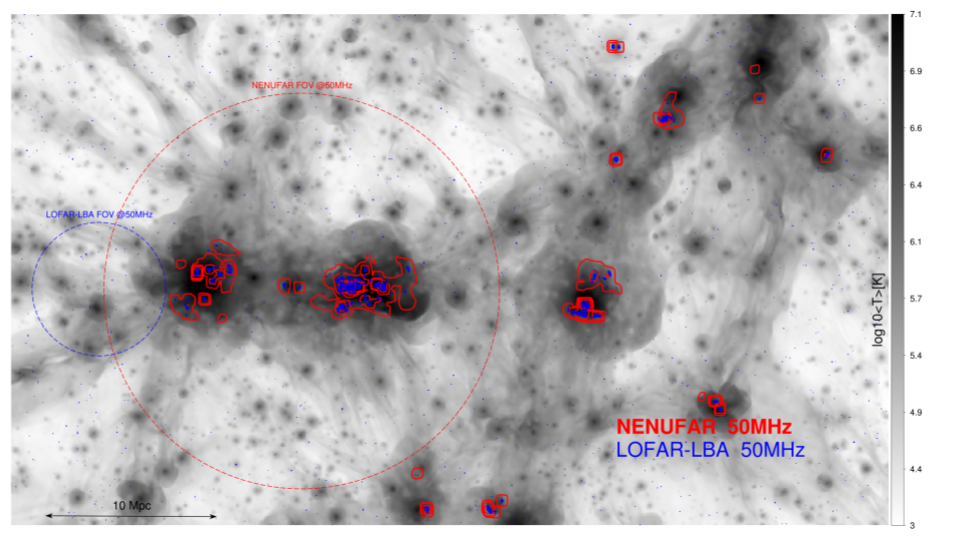
\includegraphics[width=.95\linewidth]{ProjetRecherche_futur/detection.png}
	\caption{Contours de d\'etection et champ de vue de NenuFAR et LOFAR \`a 50\,MHz. Les contours tracent la d\'etection 3$\sigma$ en l'absence d'autres sources. Figure de simulation (F. Vazza, Unibo).} \label{fig.franco.sensitivity}
\end{figure}


Mon projet de recherche se d\'eroule donc selon deux axes. D'abord, un d\'eveloppement technique et instrumental novateur, qui permettra incr\'ementalement d'atteindre de nouveaux seuils en sensibilit\'e \`a 60\,MHz. Nous y visons, chaque fois, la d\'etection du rayonnement radio-synchrotron du milieu inter-galactique dans les filaments cosmiques. Si la sensibilit\'e atteinte ne permet pas cette d\'etection, pendant le d\'eveloppement n\'ecessaire pour atteindre le prochain seuil de sensibilit\'e, nous analyserons les sources d\'etect\'ees ayant un int\'er\^et scientifique (e.g. blazars, populations de galaxies radio starburst, rayonnement fossile galactique).
La configuration observationnelle au c{\oe}ur de mon projet permettra un saut qualitatif dans la sensibilit\'e finale des relev\'es LOFAR et NenuFAR.

\newpage

\section{Mise en {\oe}uvre du programme de recherche}

\pg
Le c{\oe}ur de mon projet de recherche repose sur ma comp\'etence technique et instrumentale, que je propose de mobiliser pour contraindre l'origine cosmologique des champs magn\'etiques des filaments cosmiques. 
%Celle-ci me permet d'identifier de nouveaux modes d'utilisations porteurs pour les pr\'ecurseurs SKA en imagerie. Je propose de la mobiliser afin d'atteindre, incr\'ementalement, des limites de confusion plus ambitieuses, 
Il faudra, pour ce faire, atteindre des sensibillit\'es qui resteront in\'egal\'ees dans l'\`ere SKA. Je propose ainsi le plan suivant~:

\begin{tcolorbox}[colback=green!10, colframe=green!50!black, arc=3mm, boxrule=1pt]
\begin{enumerate}
	\item \textbf{2025}~: Atteindre la limite de confusion de NenuFAR (323\,mJy, r\'esolution $3'$);
	\item \textbf{2028}~: Atteindre 150\,$\mu$Jy \`a 60\,MHz (LOFAR + NenuFAR, r\'esolution $10''$);
	\item \textbf{2030}~: Atteindre 10\,$\mu$Jy \`a 60\,MHz (LOFAR-VLBI + NenuFAR, r\'esolution $1''$).
	\item \textbf{2034}~: Atteindre 20\,$\mu$Jy \`a 30\,MHz (LOFAR-VLBI + NenuFAR, r\'esolution $2''$).
\end{enumerate}
\end{tcolorbox}

%Chaque \'etape correspond \`a la limite finale possible avec les instruments utilis\'es~: la d\'epasser n\'ecessitera de nouveaux instruments. De surcro\^it, le passage d'une \'etape \`a la suivante permettra de valider des techniques et connaissances critiques pour l'exploitation optimale de SKA-Low.% Je d\'ecris le travail propos\'e pour chaque \'etape ci-dessous.


\subsection{Atteindre la limite de confusion de NenuFAR - amas de Coma - fin 2025}

\pg
Le projet de recherche dans son ensemble se base sur la sensibilit\'e de NenuFAR pour augmenter celle de LOFAR. La ma\^itrise technique de l'imagerie NenuFAR est donc un pr\'erequis. \`A l'heure actuelle, nous n'en sommes pas loin~: je travaille avec l'\'equipe NenuFAR pour impl\'ementer sa r\'eponse instrumentale dans des logiciels de calibration et d'imagerie qui permettront, de surcro\^it, de mitiger l'impact de l'ionosph\`ere sur la mesure. La validation de ces outils est en cours. Ils permettront \`a NenuFAR d'atteindre sa limite de confusion, de 173\,mJy \`a 66\,MHz. Cette \'etape sera la finalisation du projet pilote NenuFAR-LT09 avant le d\'eploiement d'imagerie en polarisation avec NenuFAR. %, dont les donn\'ees sont d\'ej\`a prises.

\subsection{Atteindre  150\,$\mu$Jy \`a 60\,MHz \`a 60\,MHz - M31 puis Coma - fin 2028}

\pg
La seconde \'etape est de combiner dans le plan Fourier des observations LOFAR et NenuFAR. Les donn\'ees LOFAR permettront de r\'esoudre les sources compactes d\'etect\'ees par NenuFAR, et donc d'en soustraire la contribution. Une technique similaire est utilis\'ee routinement avec le VLA \citep{1980ApJS...44..151T} et ses plusieurs configurations d'observation. Cette id\'ee peut sembler triviale, mais une fois valid\'ee, pourra permettre aux interf\'erom\`etres radio du futur de maximiser simultan\'ement leur r\'esolution angulaire et leur sensibilit\'e en exploitant cette option de combinaison h\'et\'erog\`ene dans leur conception. La validation s'effectuera sur un champ complexe mais bien \'etudi\'e, et susceptible d'inclure de l'\'emission compacte et diffuse~: celui de la galaxie d'Androm\`ede. Le but sera de d\'etecter l'\'emission diffuse de rayons cosmiques dans le halo de cette galaxie. Sa d\'etection imposerait de fortes contraintes sur certains mod\`eles d'auto-annihilation de mati\`ere noire \citep[e.g.][]{2016JCAP...11..021L,2022PhRvL.129k1103M}. \`A cette fin, nous avons obtenu, avec Thomas Seigert (JMU W\"urzburg) 1\,Ms d'int\'egration sur Androm\`ede avec INTEGRAL en rayons-$\gamma$ \citep{2003A&A...411L...1W}; 32h d'observations LOFAR, et 10h d'observations NenuFAR, \`a 60\,MHz. Je suis le PI de ces derni\`eres observations, qui ont \'et\'e prises \textit{dans le but} de valider la technique propos\'ee.%~: elle pourra donc \^etre effectu\'ee dans des d\'elais raisonnables.

\pg
Une fois valid\'ee, cette technique sera d\'eploy\'ee pour acc\'el\'erer d'un facteur 10.5 la recherche du le rayonnement radio-synchrotron des filaments cosmiques. Nous ferons une demande de temps d'observation NenuFAR afin de compl\'eter la couverture LOFAR du ciel Nord \`a 60\,MHz, dans le but d'atteindre la limite de confusion de LOFAR \`a 60\,MHz dans les champs extragalactiques. Nous poursuivrons ensuite cette approche sur tout le ciel Nord. % accessible \`a LOFAR et NenuFAR.

\subsection{Atteindre la limite de confusion de LOFAR-VLBI \`a 60\,MHz - ciel Nord - fin 2035}

\pg
La prochaine \'etape sera la r\'eduction de donn\'ees LOFAR-VLBI \`a 60\,MHz, qui est l'un des buts principaux de la collaboration Relev\'es LOFAR, et de LOFAR2.0. Ce travail se d\'eroulera sur le long terme. Ma contribution sera la prise et r\'eduction de donn\'ees NenuFAR permettant d'atteindre la limite de confusion sur tout le ciel, et le d\'eveloppement de techniques permettant le LOFAR-VLBI \`a 60\,MHz.


\subsection{Atteindre la limite de confusion de LOFAR-VLBI \`a 30\,MHz - ciel Nord - 2035+}

\pg
La fen\^etre de fr\'equence $30-50$\,MHz ne sera pas vis\'ee par le SKA. Ainsi, sur le long terme, LOFAR pourra basculer sur la cartographie du ciel radio \`a ces fr\'equences. Cela n\'ecessitera une am\'elioration de ses antennes LBA, et pourrait passer par le d\'eploiement de plusieurs stations NenuFAR-LSS dans le r\'eseau LOFAR. 

%
%
%\begin{tcolorbox}[colback=green!10, colframe=green!50!black, arc=3mm, boxrule=1pt]
%	
%LOFAR a pour ambition, \`a terme, de cartographier tout le ciel radio dans l'h\'emisph\`ere Nord. Le goulet d'\'etranglement pour ce projet est le champ de vue de l'ILT. Je propose de mener cette cartographie jusqu'\`a la limite de confusion de l'instrument, en commen\c{c}ant sur une surface restreinte, avec un but scientifique pr\'ecis~: contraindre une possible origine cosmologique des champs magn\'etiques pour lesquels nous d\'etecterons, dans le milieu inter-galactique des filaments cosmiques, une \'emission radio-synchrotron. 
%
%\end{tcolorbox}

\newpage

\section{Insertion du projet dans le paysage SKA-LOFAR}

\pg
Mon projet de recherche s'inscrit dans les travaux de relev\'es SKA et pr\'ecurseurs. Je propose un d\'eveloppement technique qui pourrait acc\'el\'erer dramatiquement ces relev\'es, et qui serait applicable \`a de futurs t\'elescopes radios. Ce d\'eveloppement est n\'ecessaire pour la r\'ealisation de mon projet de recherche.

\pg
Ce travail se situe dans le cadre de la collaboration internationale LOFAR, avec le soutien de coll\`egues en Italie (INAF et Universit\'e de Bologne), en Allemagne (GLOW, MPFiR, TLS, et JMU W\"urzburg), au Royame-Uni (Universit'es d'\'Edinbourg, de Durham, et de Manchester) et aux Pays-Bas (Universit\'e de Leydes). En France, il s'inscrit dans le cadre du d\'eveloppement de NenuFAR, men\'e \`a l'Observatoire de Paris, l'Universit\'e d'Orl\'eans, et l'Unit\'e Scientifique de Nan\c{c}ay.  L'Observatoire de Paris serait donc le lieu id\'eal o\`u mener ce projet \`a bien. L'\'equipe de Fran\c{c}oise Combes, au LERMA (UMR 8112), est particuli\`erement adapt\'ee \`a la mise en {\oe}uvre des premi\`eres \'etapes propos\'ees; j'y travaille d\'ej\`a avec Anne-Laure Melchior. Cela serait donc le cadre parfait pour mener la validation \`a moyen-terme de mon projet de recherche. La fusion des laboratoires actuels du LERMA, LUTH et GEPI sera le cadre id\'eal dans lequel le finaliser. Mes collaborations existantes avec le personnel de l'Observatoire et de l'USN (Philippe Zarka, Julien Girard, Alan Loh, Jean-Mathias Gri{\ss}meier, Cyril Tasse %TODO

\section{Impact scientifique}

\pg
La d\'etection directe d'\'emission synchrotron permettra de caract\'eriser directement, pour la premi\`ere fois, les propri\'et\'es non-thermiques du milieu inter-galactique, i.e. celles de ses composantes qui ne sont pas en \'equilibre thermodynamique avec leurs environnements. Cela permettra d'\'etudier, en-dehors des amas de galaxies, les interactions entre les jets de galaxies radio et le milieu inter-galactique. 
Si la magnitude du champ magn\'etique mesur\'e dans les filaments cosmiques est compatible avec une origine cosmologique, il sera possible d'inclure de tels champs magn\'etiques dans les mod\`eles cosmologiques. 
La cartographie de la structure magn\'etique du milieu inter-galactique dans la toile cosmique ouvrira de nouveaux horizons scientifiques. Est-ce que le champ du milieu intergalactique est ordonn\'e, et jusqu'\`a quelles \'echelles? Sont-elles super-causales, et donc n\'ecessairement form\'ees plus t\^ot durant l'expansion de l'Univers? \`A quelles \'echelles commencent les champs turbulents dans le milieu inter-galactique en-dehors des amas, et \`a quels ph\'enom\`enes astrophysiques ou cosmologiques pourraient correspondre ces \'echelles?

\pg
Quant au sc\'enario n\'egatif, de non-d\'etection d'\'emission radio-synchrotron dans le milieu inter-galactique des filaments cosmiques, il permettra d'affiner la recherche avec SKA, qui a pour un de ses buts la recherche de cette \'emission. Le projet pivotera alors sur la cr\'eation d'un relev\'e profond et efficace du ciel Nord avec la technique d\'evelopp\'ee. Les relev\'es LOFAR actuels mesurent plus de 4 millions de sources avec la sensibilit\'e actuelle \cite{2022yCat..36590001S} : je propose de d\'ecupler la sensibilit\'e finale obtenue. 
Nous \'etudierons alors les propri\'et\'es des objets recens\'es, qui inclueront galaxies radio, galaxies starburst, \'emission fossile, et nouvelles d\'ecouvertes. %De surcro\^it, LOFAR \'evite jusqu'\`a pr\'esent le plan Galactique: sur le long terme, je propose de la cartographier.
%Dans une perspective technique, %ce projet l'\'emission radio-synchrotron aux plus grandes \'echelles angulaires dans la Voie Lact\'ee.


%
%\pg
%Ainsi, dans le moyen-terme, je propose d'int\'egrer mon projet de recherche dans ces efforts \`a \'echelle internationale. Le but sera de cr\'eer des relev\'es atteignant la limite de confusion de LOFAR-VLBI en LBA, sur les r\'egions autour des amas connus. Ce projet sera limit\'e par le champ de vue de LOFAR-VLBI en LBA, de l'ordre de $\sim 2 ^\circ$. Avec le b\'en\'efice de plusieurs ann\'ees dans le LERMA, j'esp\`ere aussi pouvoir commencer \`a (co)encadrer des \'etudiants de th\`ese, qui pourront b\'en\'eficier des cartes de relev\'e produites pour ce projet pour leurs \'etudes. La formation de la prochaine g\'en\'eration d'experts LOFAR-VLBI en France pourra ainsi se faire organiquement au sein du nouveau laboratoire regroupant les \'equipes du LERMA, GEPI et LUTH actuels. 

%\pg
%Dans le long terme, le projet se d\'eclinera en fonction des r\'esultats obtenus. Avec une d\'etection du signal recherch\'e, il sera possible de tenter de cartographier la toile cosmique en radio-synchrotron dans son ensemble. Cela serait un projet de tr\`es longue dur\'ee. Sans d\'etection, le programme aura alors obtenu les meilleures limites sup\'erieures \`a ce jour sur la possibilit\'e d'un champ magn\'etique d'origine cosmologique; limites qui ne seront pas d\'epassables avec d'autres instruments au sol. Notre \'equipe se tournera vers l'exploitation scientifique des informations obtenues sur les sources d'avant-plan, qui inclueront un grand nombre de galaxies radio angulairement r\'esolues \`a tr\`es basses fr\'equences.


%
%
%Je note enfin que la m\'ethode que je propose, une fois valid\'ee, pourra \^etre appliqu\'ee au reste du ciel cartographi\'e par LOFAR~: NenuFAR permettra, de par son grand champ de vue, d'obtenir tr\`es efficacement la sensibilit\'e n\'ecessaire pour atteindre le bruit de confusion de l'ILT \`a 60\'MHz, pour tout le ciel. 

%{
%\small
%\setlength{\itemsep}{0em}
%\setlength{\parskip}{0em}
%
%\bibliographystyle{aa}
%\bibliography{bib.bib}
%}




\newpage



\chapter{Exp\'erience d'enseignement} 

\section{Enseignements effectu\'es}

\pg
Mon exp\'erience d'enseignement est d\'ecrite succinctement dans \cref{CV}. J'en r\'esume les caract\'eristiques dans la \cref{tab.teaching}; NASSP signifie "National Astrophysics and Space Science Programme", une structure Sud-Africaine. J'ai \'et\'e charg\'e d'une mission d'enseignement durant ma th\`ese, mais celle-ci ne s'est d\'eroul\'ee qu'a moiti\'e en France; je n'ai donc que 96 heures d'ETD \`a mon actif dans le cadre de cette mission. J'ai compl\'et\'e mon enseignement de ma propre initiative durant mes \'etudes en Afrique du Sud.

\begin{table}[h!]
	\begin{tabular}{|c|c|c|c|}
		\hline
		Enseignement & Institution & Niveau & eHTD \\ \hline 
		Introduction \`a la physique & Rhodes University, Afrique du Sud & L1 & 60 \\ 
		Interf\'erom\'etrie & NASSP, Afrique du Sud & M2 & 15 \\
		Lumi\`eres sur l'Univers & Observatoire de Paris & Dipl\^ome d'Universit\'e & 60 \\
		TP Observation & Unit\'e Scientifique de Nan\c{c}ay & M2 & 20 \\
		Parrainage & Observatoire de Paris & \'Ecole et coll\`ege & 15 \\ \hline
	\end{tabular}\label{tab.teaching}
%\caption{balbla }
\end{table}

\section{Approche p\'edagogique}

\pg
J'ai fait mes \'etudes dans le cadre de plusieurs syst\`emes \'educatifs: syst\`eme Fran\c{c}ais et CNED jusqu'au coll\`ege, syst\`eme Am\'ericain au Bac, licence dans le syst\`eme \'ecossais, et Master \`a l'Observatoire de Paris en France. Chacun a mobilis\'e une approche p\'edagogique propre, en mettant l'emphase sur diff\'erents aspects des concepts enseign\'es.
J'ai de surcro\^it enseign\'e dans le secondaire en Afrique du Sud, au niveau de la L1. Cette exp\'erience a compris \`a la fois encadrement de TDs et cours magistraux. 

\pg
Fort de ces exp\'eriences, je consid\`ere qu'un enseignement efficace demande une forte organisation, qui est une condition n\'ecessaire pour rendre les concepts transmis le plus clair possible, naviguer les doutes et confusions des \'etudiants, et leur permettre de synth\'etiser efficacement leurs connaissances nouvelles avec leur compr\'ehension existante. Bien qu'une telle organisation demande beaucoup de temps, de travail et de discipline, elle permet de faciliter \'enorm\'ement la t\^ache d'enseignement pour tous, professeurs et \'etudiants, une fois men\'ee \`a bien.

\pg
Elle n'est cependant pas suffisante: je consid\`ere qu'il est critique de savoir communiquer \`a ses \'etudiants notre propre int\'er\^et pour la physique, aussi bien sa technique que sa science. Il existe de nombreuses barri\`eres \`a l'assimilation efficace de connaissances: celles-ci peuvent relever de l'ordre de contraintes sociales (e.g. projets d'enfants ou responsabilit\'es de garde de d\'ependants), mat\'erielles (e.g. n\'ecessit\'e de gagner sa vie), psychologiques (e.g. \'episodes de d\'epression chronique), etc. Faire du travail d'assimilation de connaissances un fardeau maximisera les chances que son succ\`es se heurtera \`a ces barri\`eres. Je pense que la meilleure fa\c{c}on de permettre aux \'etudiants de s'approprier r\'eellement le contenu de leurs cours est, d'abord, de leur \textit{donner confiance} en leur propres capacit\'es. 

\pg
La seconde partie du travail d'enseignant revient alors a demander aux \'etudiants de confronter les limites de leur compr\'ehension dans le but d'apprendre. C'est l\`a que l'int\'er\^et pour les sujets abord\'es peut \^etre transmis, que ce soit durant les cours, en travaux dirig\'es ou en travaux pratiques. En communiquant aux \'etudiants que les probl\`emes auxquels ils font face sont r\'esolvables, qu'ils sont capables de les confronter, mais que cela demande un travail dont la gratification est le d\'eveloppement de soi et de leurs connaissances, il devient possible de leur communiquer une motivation propre \`a s'investir dans leur formation, en plus de celles qui les auront pouss\'es \`a la rejoindre (si ce n'\'etait pas leur motivation principale). 

\pg
Mon approche p\'edagogique consiste donc \`a prendre tr\`es au s\'erieux la demande d'organisation impos\'ee par des devoirs d'enseignement. J'{\oe}uvre ensuite \`a permettre aux \'etudiants de se sentir en confiance (e.g. oser poser des questions ``b\^etes'', discuter entre eux des sujets enseign\'es, etc), pour leur communiquer les concepts \`a enseigner de fa\c{c}on \`a les encourager \`a devenir moteurs de leur travail. Ceci fait, le travail p\'edagogique devient un travail d'encadrement et de communication. Je note au passage qu'il y aura certainement des \'etudiants qui se sentiront d\'ej\`a en confiance, auront la capacit\'e de travail n\'ecessaire pour mener leur formation \`a bien, et feront des \'etudes formidables. Ma priorit\'e est de permettre aux \'etudiants qui ne font pas encore partie de cette cohorte de la rejoindre en cours de route. Ensuite, je personne ne pourra apprendre \`a leur place: je ne peux que les encadrer.


\section{Encadrement de projets de Master et de th\`ese}

\pg
J'ai eu la chance de pouvoir encadrer de nombreux travaux d'\'etudiants de Master et de th\`ese. Durant mon premier poste post-doctoral \`a l'Universit\'e de Bologne, je me suis fait confier l'encadrement de la r\'eduction de donn\'ees LOFAR de plusieurs \'etudiants en Master, Noemi Labella et Giada Pignatora. Cette derni\`ere a poursuivi sa recherche en th\`ese dans la m\^eme \'equipe. J'ai de plus eu la responsabilit\'e d'encadrer la r\'eduction de donn\'ees de deux th\'esards dans la m\^eme p\'eriode, Nadia Biava (qui a d\'efendu sa th\`ese en 2021) et Giada Pignatora.

\pg
Dans le cadre de mon second poste post-doctoral \`a l'Universit\'e de W\"urzburg, je me suis fait confier l'encadrement du projet de th\`ese de Hrishikesh Shetgaonkar, dont le contrat commen\c{c}ait dans la m\^eme p\'eriode que le mienne. Ma responsabilit\'e rel\`eve \`a la fois de l'encadrement au jour le jour (mise \`a niveau technique, discussions scientifiques, et aide \`a la prise de confiance) et du transfert de connaissances et d'expertise technique (d\'eveloppement de pipelines de r\'eduction, capacit\'e de diagnostic d'images radio-interf\'erom\'etriques, et expertise dans la r\'eduction artisanale de donn\'ees radio). Il entame maintenant sa troisi\`eme ann\'ee de th\`ese, sur un total de quatre pr\'evues, avec deux publications scientifiques en cours de r\'edaction, et ayant pr\'esent\'e ses travaux dans de nombreuses conf\'erences nationales et internationales. 

\pg
Je me suis enfin fait confier l'encadrement d'un \'etudiant en Erasmus \`a l'Universit\'e de W\"urzburg, qui commencera son m\'emoire de Master dans notre \'equipe dans le printemps. J'ai moi-m\^eme \'elabor\'e son projet, qui portera sur la mise en {\oe}uvre d'une technique radio-interf\'erom\'etrique novatrice. 

\section{Insertion dans la Facult\'e de Physique}

\pg
J'ai contact\'e plusieurs personnels de la Facult\'e de Physique (J\'er\^ome Tignon, Pac\^ome Delva, Gwena\"el Bou\'e) afin d'avoir une id\'ee des besoins d'enseignements, ainsi que des projets d\'ej\`a en place. Si ma candidature est retenue, je me plierai \'evidemment aux besoins de la Facult\'e de Physique, en particulier en termes de gestions de groupes de TD et pour l'encadrement du programme de r\'esolution de probl\`emes. Fort de mon exp\'erience au DU-LU de l'Observatoire, je pense que je serai tout \`a fait capable de participer aussi \`a la formation num\'erique de python sur jupyterhubb propos\'ee en L1. Enfin, je peux participer \`a la r\'edaction de documents centraux n\'ecessaires \`a une organisation et une communication efficace entre tout le personnel d'enseignement (polycopi\'es, biblioth\`eque de simulations, cr\'eation d'interfaces utilisateurs agr\'eables, etc), en mettant l'emphase sur la centralit\'e des fondamentaux (physique, math\'ematiques, informatique) qui permettront aux \'etudiants de la Facult\'e de poursuivre sereinement leurs projets professionnels, dans la recherche ou l'industrie.

\pg
Je suis conscient de la charge de travail que repr\'esente la t\^ache d'enseignement du statut de ma\^itre de conf\'erences - m\^eme avec la d\'echarge de premi\`ere ann\'ee prise en compte. J'esp\`ere pouvoir, si possible, utiliser la d\'echarge de 32h ETD des 5 premi\`eres ann\'ees de statut afin de suivre des formations de p\'edagogie pour obtenir, si possible, CAPES et aggr\'egation. Ce projet ne sera poursuivi, \'evidemment, qu'avec le soutien de la Facult\'e de Physique.

\begin{tcolorbox}[colback=green!10, colframe=green!50!black, arc=3mm, boxrule=1pt]
	Mon profil d'enseignement est adapt\'e aux besoins de la Facult\'e de Physique de Sorbonne-Universit\'e: j'ai \`a la fois une exp\'erience d'encadrement de TD/TP, de suivi num\'erique \`a distance, et d'\'elaboration de documents p\'edagogiques de type jupyter notebook. L'investissement de Sorbonne-Universit\'e dans des m\'ethodes p\'edagogiques novatrices (enseignement agile, atelier de recherche encadr\'ee, r\'esolution de probl\`emes) m'int\'eresse \'enorm\'ement: j'esp\`ere avoir l'occasion de les d\'eployer moi-m\^eme.
\end{tcolorbox}










\newpage



\chapter{Temps d'observation obtenus sur t\'elescopes} 

\pg
Mon profil de recherche est celui d'un observateur. J'ai d\'evelopp\'e une capacit\'e \`a identifier des besoins observationnels pour divers projets scientifiques, et d'obtenir le temps d'observation n\'ecessaire. J'ai non seulement obtenu du temps d'observation pour mes propres projets scientifiques, mais aussi en soutien \`a des projets d'\'etudiants en th\`ese.

\pg
J'ai obtenu le temps d'observation en PI (Primary Investigator) sur les projets suivant:
\begin{itemize}
	\item Un total de 60h d'observations NenuFAR dans le cadre du projet LT09 ``Magn\'etisme et Filaments Cosmiques", dont je suis le Principal Investigator.
	\item Un total de 10h d'observations NenuFAR sur M31 (code RP2A), la galaxie d'Androm\`ede, afin de d\'etecter le rayonnement radio-synchrotron provenant de son halo.
	\item Un total de 32h d'observations de M31 avec LOFAR dans sa bande LBA, \`a 60\,MHz, afin de compl\'eter la couverture spectrale de cette source.
	\item Un total de 4h d'observations sur une source myst\'erieuse afin d'en d\'eterminer la nature. Celle-ci se trouvait en bord de champ d'une observation NenuFAR de M31.
	\item Un total de 30h d'observations de M31 avec l'uGMRT (proposal ID 46\_082) .
	\item Un total de 192h sur NenuFAR et sur l'International LOFAR Telescope (ILT, i.e. LOFAR avec lignes de bases internationales) afin de mener \`a bien le commissioning du mode NenuFAR-LSS.
\end{itemize}

\pg
J'ai de plus \'et\'e Co-I sur les projets suivants:
\begin{itemize}
	\item 1Ms d'observations avec INTEGRAL (ID: 2120016) sur M31. Ce projet a \'et\'e men\'e par un coll\`egue, Thomas Siegert, dans le but de compl\'eter en gamma la couverture radio obtenue la m\^eme ann\'ee.
	\item 7h d'observations MeerKAT portant sur des observations de suivi de d\'etections IceCUBE (neutrinos), dans le but d'en d\'eterminer l'origine. Ce projet a \'et\'e \'elabor\'e par moi-m\^eme ainsi qu'un \'etudiant de th\`ese \`a l'Universit\'e de W\"urzburg, Florian R\"osch.
	\item 20h d'observations MeerKAT portant sur le suivi d'un sursaut gamma, dans le but d'en d\'eterminer l'origine par imagerie radio. Ce projet a \'et\'e \'elabor\'e et men\'e par Florian Eppel, un th\'esard \`a l'Universit\'e de W\"urzburg: j'ai servi de soutien et d'expert technique.
	\item 11h d'observations uGMRT sur le blazar 4C+19.44 (proposal ID 46\_081). Ce projet a \'et\'e men\'e par mon \'etudiant en th\`ese, qui \'etudie les n{\oe}uds du jet de ce blazar \`a basses fr\'equences.
	\item 60h d'observations LOFAR-VLBI de blazars \'emettant en TeV (ProjID: LC20\_033), pour un projet men\'e par mon \'etudiant en th\`ese, Hrishikesh Shetgaonkar. Ces observations lui permettront d'\'elaborer une \'etude de population de la contrepartie radio de ces jets gamma.
	\item 26h d'observations LOFAR-HBA d'une population d'amas de galaxies \`a mini-halos (ProjID: LC16\_003), pour un projet men\'e par mon coll\`egue Christopher Riseley afin de d\'eterminer leurs propri\'et\'es spectrales avec LOFAR et MeerKAT. 
	\item 38 d'observations LOFAR-HBA de diff\'erents amas (ProjID: LC15\_021), pour un projet men\'e par ma coll\`egue Kamlesh Rajpurohit dans le but d'\'etudier une classe de reliques radio dont l'\'emissin serait g\'en\'er\'ee principalement par le m\'ecanisme de Diffusive Shock Acceleration.
	\item 80h d'observations LOFAR-HBA de l'amas de Coma (ProjID: LC15\_020), por un projet men\'e par Annalisa Bonafede, cheffe du groupe de recherche dans lequel j'ai travaill\'e pour mon premier post-doc \`a Bologne. J'ai servi d'expertise technique pour ce projet.
	\item 10h d'observations LOFAR-LBA de l'amas cool-core RXJ1720.1+2638 (ProjID: LC12\_018). Ce projet a \'et\'e men\'e par Nadia Biava durant sa th\`ese \`a l'Universit\'e de Bologne.
\end{itemize}

\pg
Je suis donc capable d'obtenir, de fa\c{c}on fiable, du temps d'observation sur des t\'elescopes de classe pr\'ecurseurs SKA, pour mes propres projet, en soutien \`a ceux de mes coll\`egues, ou bien pour des projets de th\`eses.








\newpage
\chapter{Travaux d'instrumentation} 

\pg



\end{document}
